\chapter{Introduction to Trigonometry}
Reading Materials: \newline
Croft, A. and R. Davidson \textit{Foundation maths.} (Harlow: Pearson, 2016) 6th edition. \textbf{Chapter 22 Introduction to trigonometry.}

\vspace{5mm}

\noindent An \textbf{angle $\theta$} is a measure of separation of two rays emanating from \textbf{vertex $v$}.

\begin{figure}[htp]
	\centering
	
\includegraphics[width=\linewidth]{Assets/angles}
	\caption{angle formed by rays A and B from a vertex}
	\label{fig:angles}
\end{figure}

\noindent It is measured in degrees or radians.

\vspace{5mm}

\noindent One radian is the angle between two radii. that intercept on the circumference and arc of the same length of the radius.

\begin{equation}
	2 \pi \text{ radians} = 360^{\circ}
\end{equation}

\begin{figure}[htp]
	\centering
	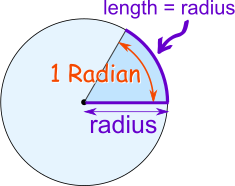
\includegraphics[width=50mm]{Assets/radian-circle}
	\caption{definition of radian}
	\label{fig:radian}
\end{figure}
\newpage
\section{Right Angle Triangle Properties}
\begin{figure}[htp]
	\centering
	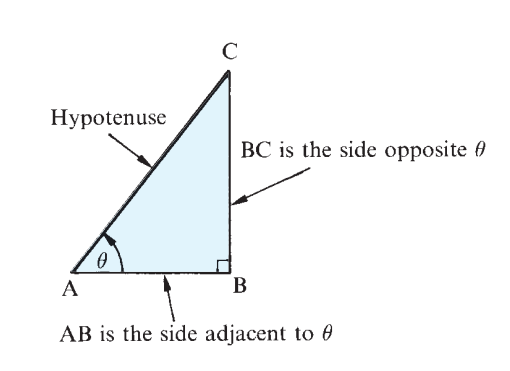
\includegraphics[width=75mm]{Assets/right-angle-triangle}
	\caption{a right angle triangle}
	\label{fig:right-angle}
\end{figure}
\noindent The side opposite the right angle is always called the hypotenuse. So,
in Figure 4.3 the hypotenuse is AC. The side opposite $\theta$ is BC. The
remaining side, AB, is said to be adjacent to $\theta$. Then we have for angle $\theta$ we have the trigonometric ratios:
\begin{equation} \label{eq1}
	\begin{split}
		\sin\theta & = \frac{\text{opposite}}{\text{hypotenuse}} = \frac{\text{BC}}{\text{AC}} \\
		\cos\theta & = \frac{\text{adjacent}}{\text{hypotenuse}} = \frac{\text{AB}}{\text{AC}} \\
		\tan\theta & = \frac{\text{opposite}}{\text{adjacent}} = \frac{\text{BC}}{\text{AB}}
	\end{split}
\end{equation}
\section{Similar Triangle}
\begin{figure}[htp]
	\centering
	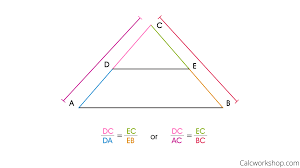
\includegraphics{Assets/similar-triangle}
	\caption{similar triangle}
	\label{fig:radian}
\end{figure}
\section{Examples}